% interactcadsample.tex
% v1.03 - April 2017

\documentclass[]{interact}

\usepackage{epstopdf}% To incorporate .eps illustrations using PDFLaTeX, etc.
\usepackage{subfigure}% Support for small, `sub' figures and tables
%\usepackage[nolists,tablesfirst]{endfloat}% To `separate' figures and tables from text if required

\usepackage{natbib}% Citation support using natbib.sty
\bibpunct[, ]{(}{)}{;}{a}{}{,}% Citation support using natbib.sty
\renewcommand\bibfont{\fontsize{10}{12}\selectfont}% Bibliography support using natbib.sty

\theoremstyle{plain}% Theorem-like structures provided by amsthm.sty
\newtheorem{theorem}{Theorem}[section]
\newtheorem{lemma}[theorem]{Lemma}
\newtheorem{corollary}[theorem]{Corollary}
\newtheorem{proposition}[theorem]{Proposition}

\theoremstyle{definition}
\newtheorem{definition}[theorem]{Definition}
\newtheorem{example}[theorem]{Example}

\theoremstyle{remark}
\newtheorem{remark}{Remark}
\newtheorem{notation}{Notation}


% tightlist command for lists without linebreak
\providecommand{\tightlist}{%
  \setlength{\itemsep}{0pt}\setlength{\parskip}{0pt}}



\usepackage{lscape}
\usepackage{hyperref}
\usepackage[utf8]{inputenc}
\def\tightlist{}

\usepackage{booktabs}
\usepackage{longtable}
\usepackage{array}
\usepackage{multirow}
\usepackage{wrapfig}
\usepackage{float}
\usepackage{colortbl}
\usepackage{pdflscape}
\usepackage{tabu}
\usepackage{threeparttable}
\usepackage{threeparttablex}
\usepackage[normalem]{ulem}
\usepackage{makecell}
\usepackage{xcolor}

\begin{document}


\articletype{}

\title{Appendix: A Plot is Worth a Thousand Tests: Assessing Residual
Diagnostics with the Lineup Protocol}


\author{\name{Weihao Li$^{a}$, Dianne Cook$^{a}$, Emi
Tanaka$^{a}$, Susan VanderPlas$^{b}$}
\affil{$^{a}$Department of Econometrics and Business Statistics, Monash
University, Clayton, VIC, Australia; $^{b}$Department of Statistics,
University of Nebraska, Lincoln, Nebraska, USA}
}

\thanks{CONTACT Weihao
Li. Email: \href{mailto:weihao.li@monash.edu}{\nolinkurl{weihao.li@monash.edu}}, Dianne
Cook. Email: \href{mailto:dicook@monash.edu}{\nolinkurl{dicook@monash.edu}}, Emi
Tanaka. Email: \href{mailto:emi.tanaka@monash.edu}{\nolinkurl{emi.tanaka@monash.edu}}, Susan
VanderPlas. Email: \href{mailto:susan.vanderplas@unl.edu}{\nolinkurl{susan.vanderplas@unl.edu}}}

\maketitle



\appendix

\hypertarget{additional-details-of-testing-procedures}{%
\section{Additional details of testing
procedures}\label{additional-details-of-testing-procedures}}

\hypertarget{effect-size-derivation}{%
\subsection{Effect size derivation}\label{effect-size-derivation}}

Effect size can be defined as the difference of a parameter for a
particular model or distribution, or a statistic derived from a sample.
Importantly, it needs to reflect the treatment we try to measure.
Centred on a conventional statistical test, we usually can deduce the
effect size from the test statistic by substituting the null parameter
value. When considering the diagnostics of residual departures, there
exist many possibilities of test statistics for a variety of model
assumptions. Meanwhile, diagnostic plots such as the residual plot have
no general agreement on measuring how strong a model violation pattern
is. To build a bridge between various residual-based tests, and the
visual test, we focus on the shared information embedded in the testing
procedures, which is the distribution of residuals. When comes to
comparison of distribution, Kullback-Leibler divergence
\citep{kullback1951information} is a classical way to represent the
information loss or entropy increase caused by the approximation to the
true distribution, which in our case, the inefficiency due to the use of
false model assumptions.

Following the terminology introduced by \citet{kullback1951information},
\(P\) represents the measured probability distribution, and \(Q\)
represents the assumed probability distribution. The Kullback-Leibler
divergence is defined as
\(\int_{-\infty}^{\infty}log(p(x)/q(x))p(x)dx\), where \(p(.)\) and
\(q(.)\) denote probability densities of \(P\) and \(Q\).

Let \(\boldsymbol{X}\) denotes the \(p + 1\) regressors with \(n\)
observations,
\(\boldsymbol{b} = (\boldsymbol{X}'\boldsymbol{X})^{-1}\boldsymbol{X}'\boldsymbol{y}\)
denotes the OLS solution,
\(\boldsymbol{R} = \boldsymbol{I}_n -\boldsymbol{X}(\boldsymbol{X}'\boldsymbol{X})^{-1}\boldsymbol{X}'\)
denotes the residual operator, and let
\(\boldsymbol{\varepsilon} \sim N(\boldsymbol{0},\sigma^2\boldsymbol{I})\)
denotes the error. The residual vector

\begin{align*}
\boldsymbol{e} &= \boldsymbol{y} - \boldsymbol{X}\boldsymbol{b} \\
               &= \boldsymbol{y} - \boldsymbol{X}(\boldsymbol{X}'\boldsymbol{X})^{-1}\boldsymbol{X}'\boldsymbol{y} \\
               &= (\boldsymbol{I} -\boldsymbol{X}(\boldsymbol{X}'\boldsymbol{X})^{-1}\boldsymbol{X}')\boldsymbol{y} \\
               &= \boldsymbol{R}\boldsymbol{y} \\
               &= \boldsymbol{R}(\boldsymbol{X}\boldsymbol{\beta} + \boldsymbol{\varepsilon}) \\
               &= \boldsymbol{R}\boldsymbol{\varepsilon}.
\end{align*}

Because \(rank(\boldsymbol{R}) = n - p - 1 < n\), \(\boldsymbol{e}\)
follows a degenerate multivariate normal distribution and does not have
a density. Since the Kullback-Leibler divergence requires a proper
density function, we need to simplify the covariance matrix of
\(\boldsymbol{e}\) by setting all the off-diagonal elements to 0. Then,
the residuals will assumed to follow
\(N(\boldsymbol{0}, diag(\boldsymbol{R}\sigma^2))\) under the null
hypothesis that the model is correctly specified. If the model is
however misspecified due to omitted variables \(\boldsymbol{Z}\), or a
non-constant variance \(\boldsymbol{V}\), the distribution of residuals
can be derived as
\(N(\boldsymbol{R}\boldsymbol{Z}\boldsymbol{\beta}_z, diag(\boldsymbol{R}\sigma^2))\)
and
\(N(\boldsymbol{0}, diag(\boldsymbol{R}\boldsymbol{V}\boldsymbol{R}'))\)
respectively.

By assuming both \(P\) and \(Q\) are multivariate normal density
functions, the Kullback-Leibler divergence can be rewritten as
\[KL = \frac{1}{2}\left(log\frac{|\Sigma_p|}{|\Sigma_q|} - n + tr(\Sigma_p^{-1}\Sigma_q) + (\mu_p - \mu_q)'\Sigma_p^{-1}(\mu_p - \mu_q)\right).\]

Then, we can combine the two residual departures into one formula

\small

\begin{equation*}
\label{eq:effect-size}
KL = \frac{1}{2}\left(log\frac{|diag(\boldsymbol{R}\boldsymbol{V}\boldsymbol{R}')|}{|diag(\boldsymbol{R}\sigma^2)|} - n + tr(diag(\boldsymbol{R}\boldsymbol{V}\boldsymbol{R}')^{-1}diag(\boldsymbol{R}\sigma^2)) + \boldsymbol{\mu}_z^{T}(\boldsymbol{R}\boldsymbol{V}\boldsymbol{R}')^{-1}\boldsymbol{\mu}_z\right).
\end{equation*}

\normalsize

When there are omitted variables but constant error variance, the
formula can be reduced to

\[KL = \frac{1}{2}\left(\boldsymbol{\mu}_z^{T}(diag(\boldsymbol{R}\sigma^2))^{-1}\boldsymbol{\mu}_z\right).\]

And when the model equation is correctly specified but the error
variance is non-constant, the formula can be reduced to

\[KL = \frac{1}{2}\left(log\frac{|diag(\boldsymbol{R}\boldsymbol{V}\boldsymbol{R}')|}{|diag(\boldsymbol{R}\sigma^2)|} - n + tr(diag(\boldsymbol{R}\boldsymbol{V}\boldsymbol{R}')^{-1}diag(\boldsymbol{R}\sigma^2))\right).\]
Since we assume \(\sigma = 1\) for the heteroskedasticity model, the
final form of the formula is

\[KL = \frac{1}{2}\left(log\frac{|diag(\boldsymbol{R}\boldsymbol{V}\boldsymbol{R}')|}{|diag(\boldsymbol{R})|} - n + tr(diag(\boldsymbol{R}\boldsymbol{V}\boldsymbol{R}')^{-1}diag(\boldsymbol{R}))\right).\]

\hypertarget{sensitivity-analysis-for-alpha}{%
\subsection{\texorpdfstring{Sensitivity analysis for
\(\alpha\)}{Sensitivity analysis for \textbackslash alpha}}\label{sensitivity-analysis-for-alpha}}

The parameter \(\alpha\) used for the \(p\)-value calculation needs to
be estimated from responses to null lineups. With a greater value of
\(\hat{\alpha}\), the \(p\)-value will be smaller, resulting in more
lineups being rejected. However, The way we generate Rorschach lineup is
not strictly the same as what suggested in
\citet{vanderplas2021statistical} and \citet{buja_statistical_2009}.
Therefore, we conduct a sensitivity analysis in this section to examine
the impact of the variation of the estimator \(\alpha\) on our primary
findings.

The analysis is conducted by setting up several scenarios, where the
\(\alpha\) is under or overestimated by 12.5\%, 25\% and 50\%. Using the
adjusted \(\hat{\alpha}\), we recalculate the \(p\)-value for every
lineup and show the results in Figure \ref{fig:sensitivity}. It can be
observed that there are some changes to \(p\)-values, especially when
the \(\hat{\alpha}\) is multiplied by 50\%. However, Table
\ref{tab:sensitivity} shows that adjusting \(\hat{\alpha}\) will not
result in a huge difference in rejection decisions. There are only a
small percentage of cases where the rejection decision change. It is
very unlikely the downstream findings will be affected because of the
estimate of \(\alpha\).

\begin{figure}

{\centering \includegraphics[width=1\linewidth]{appendix_files/figure-latex/sensitivity-1} 

}

\caption{Change of $p$-values with $\hat{\alpha}$ multiplied by $0.5$, $0.75$, $0.875$, $1.125$, $1.25$ and $1.5$. Only lineups with uniform fitted value distribution is used. The vertical dashed line indicates $p\text{-value} = 0.05$. The area coloured in red indicates $\text{adjusted }p\text{-value} < 0.05$. The x-axis is drawn on logarithmic scale. For multipliers smaller than 1, the adjusted $p\text{-value}$ will initially increase and decline when the $p\text{-value}$ increases. The trend is opposite with multipliers greater than $1$, but the difference eventually reaches $0$.}\label{fig:sensitivity}
\end{figure}

\begin{table}

\caption{\label{tab:sensitivity}Examining how decisions might change if $\hat{\alpha}$ was different. Percentage of lineups that where the $p$-value would switch to above or below 0.05, when $\hat{\alpha}$ is multiplied by a multiplier.}
\centering
\begin{tabular}[t]{rrrrr}
\toprule
Multiplier & Reject to not reject & \% & Not reject to reject & \%\\
\midrule
0.500 & 7 & 2.51 & 0 & 0.00\\
0.750 & 4 & 1.43 & 0 & 0.00\\
0.875 & 3 & 1.08 & 0 & 0.00\\
\addlinespace
1.125 & 0 & 0.00 & 3 & 1.08\\
1.250 & 0 & 0.00 & 4 & 1.43\\
1.500 & 0 & 0.00 & 5 & 1.79\\
\bottomrule
\end{tabular}
\end{table}

\hypertarget{effect-of-number-of-evaluations-on-the-power-of-a-visual-test}{%
\subsection{Effect of number of evaluations on the power of a visual
test}\label{effect-of-number-of-evaluations-on-the-power-of-a-visual-test}}

When comparing power of visual tests across different fitted value
distributions, we have discussed the number of evaluations on a lineup
will affect the power of the visual test. Using the lineups with uniform
fitted value distribution, we show in Figure \ref{fig:n_eval} the change
of power of visual tests due to different number of evaluations. It can
be learned that as the number of evaluations increases, the power will
increase but the margin will decrease. Considering we have eleven
evaluations on lineups with uniform fitted value distribution, and five
evaluations on other lineups, it is necessary to use the same number of
evaluations for each lineup in comparison.

\begin{figure}

{\centering \includegraphics[width=0.7\linewidth]{appendix_files/figure-latex/n_eval-1} 

}

\caption{Change of power of visual tests for different number of evalutions on lineups with uniform fitted value distribution. The power will increase as the number of evaluations increases, but the margin will decrease.}\label{fig:n_eval}
\end{figure}

\hypertarget{power-of-a-reset-test-under-different-auxiliary-regression-formulas}{%
\subsection{Power of a RESET test under different auxiliary regression
formulas}\label{power-of-a-reset-test-under-different-auxiliary-regression-formulas}}

It is found in the result that the power of a RESET test will be
affected by the highest order of fitted values included in the auxiliary
formula. And we suspect that the current recommendation of the highest
order - four, is insufficient to test complex non-linear structures such
as the ``Triple-U'' shape designed in this paper. Figure \ref{fig:reset}
illustrates the change of power of RESET test while testing the ``U''
shape and the ``Triple-U'' shape with different highest orders. Clearly,
when testing a simple shape like the ``U'' shape, the highest order has
very little impact on the power. But for testing the ``Triple-U'' shape,
there will be a loss of power if the recommended order is used. To avoid
the loss of power, the highest order needs to be set to at least six.

\begin{figure}

{\centering \includegraphics[width=1\linewidth]{appendix_files/figure-latex/reset-1} 

}

\caption{Change of power of RESET tests for different orders of fitted values included in the auxiliary formula. The left panel is the power of testing the "U" shape and the right panel is the power of testing the "Triple-U" shape. The power will not be greatly affected by the highest order in the case of testing the "U" shape. In the case of testing the "Triple-U" shape, the highest order needs to be set to at least six to avoid the loss of power.}\label{fig:reset}
\end{figure}

\hypertarget{conventional-test-rejection-rate-for-varying-significance-levels}{%
\subsection{Conventional test rejection rate for varying significance
levels}\label{conventional-test-rejection-rate-for-varying-significance-levels}}

In the main paper, Sections 5.1 and 5.2 compared the power, and the
decisions made by the conventional tests and the visual test. The power
curves for the visual test is effectively a right-shift from the
conventional test. The effect is that the visual test rejects less often
than the conventional test, at the same significance level. We also saw
that the visual test rejected a subset of those that the conventional
tests rejected. This means that they agreed quite well - only residual
plots rejected by the contentional tests were rejected by the visual
test. There was little disagreement, where residual plots not rejected
by the conventional test were rejected by the visual test. The question
arises whether the decisions made conventional test could be made
similar to that of the visual test by reducing the significance level.
Reducing the significance level from 0.05, to 0.01, 0.001, \ldots{} will
have the effect of rejecting fewer of the residual plots.

It would be interesting if a different conventional test significance
level results in both the visual tests and conventional tests reject
only the same residual plots, and fails to reject the same residual
plots. This would be a state where both systems agree perfectly. Figure
\ref{fig:rej-rates} examines this. Plot A shows the percentage of
residual plots rejected by the visual test, given the conventional test
rejected (solid lines) or failed to reject (dashed lines). The vertical
grey line marks significance level 0.05. When the signicance level gets
smaller, the it is possible te see that the visual tests reject (nearly)
100\% of the time that the conventional test rejects. However, there is
not agreement, because the visual tests also increasingly reject
residual plots where the conventional test failed to reject. Plot B is
comparable to an ROC curve, where the percentage visual test rejection
conditional on conventional test decision is plotted: Reject conditional
on reject is plotted against reject conditional on fail to reject, for
different significance levels. The non-linearity pattern results are
close to being ideal, that the percentage of reject relative to fail to
reject increases very slowly as the reject relative to reject converges
to 100. The heteroskedasticity pattern is more problematic, and shows
that the cost of rejecting less with the conventional test is
disagreement with the visual test.

\begin{figure}[t!]

{\centering \includegraphics[width=1\linewidth]{appendix_files/figure-latex/rej-rates-1} 

}

\caption{Changing the significance level of the conventional test will change the rejection rate. A: Percentage of conventional tests also rejected by the visual test: rejected (solid), not rejected (dashed). As the significance level is reduced, the percentage rejected by the visual test that has been rejected by the conventional test approaches 100. The percentage of tests not rejected by the conventional test also increases, as expected, but the percentage of these that are rejected by the visual test increases too. B: ROC curve shows that forcing the conventional test to not reject creates a discrepancy with the visual test. Many of the residual plots not rejected by the conventional test are rejected by the visual test. It isn't possible to vary the significance level of the conventional test to match the decisions made by the visual test.}\label{fig:rej-rates}
\end{figure}

\hypertarget{experiment-setup}{%
\section{Experiment setup}\label{experiment-setup}}

\hypertarget{mapping-of-participants-to-experimental-factors}{%
\subsection{Mapping of participants to experimental
factors}\label{mapping-of-participants-to-experimental-factors}}

Mapping of participants to experimental factors is an important part of
experiment design. Essentially, we want to maximum the difference in
factors exposed to a participant. For this purpose, we design an
algorithm to conduct participant allocation. Let \(L\) be a set of
available lineups and \(S\) be a set of available participants.
According to the experimental design, the availability of a lineup is
associated with the number of participants it can assign to. For lineups
with uniform fitted value distribution, this value is 11. And other
lineups can be allocated to at most five different participants. The
availability of a participant is associated with the number of lineups
that being allocated to this participant. A participant can view at most
18 different lineups.

The algorithm starts from picking a random participant \(s \in S\) with
the minimum number of allocated lineups. It then tries to find a lineup
\(l \in L\) that can maximise the distance metric \(D\) and allocate it
to participant \(s\). Set \(L\) and \(S\) will be updated and the
picking process will be repeated until there is no available lineups or
participants.

Let \(F_1,...,F_q\) be \(q\) experimental factors, and \(f_1, ...,f_q\)
be the corresponding factor values. We say \(f_i\) exists in \(L_{s}\)
if any lineup in \(L_{s}\) has this factor value. Similarly, \(f_if_j\)
exists in \(L_{s}\) if any lineup in \(L_{s}\) has this pair of factor
values. And \(f_if_jf_k\) exists in \(L_{s}\) if any lineup in \(L_{s}\)
has this trio of factor values. The distance metric \(D\) is defined
between a lineup \(l\) and a set of lineups \(L_{s}\) allocated to a
participant \(s\) if \(L_{s}\) is non-empty:

\footnotesize

\begin{equation*}
D =
C - \sum_{1\leq i \leq q}I(f_i\text{ exists in }L_{s}) - \sum_{\substack{1\leq i \leq q-1 \\ i < j \leq q}}I(f_if_j\text{ exists in }L_{s}) - \sum_{\substack{1\leq i \leq q - 2 \\ i < j \leq q - 1 \\ j < k \leq q}}I(f_if_jf_k\text{ exists in }L_{s})
\end{equation*}

\normalsize

where \(C\) is a sufficiently large constant such that \(D > 0\). If
\(L_{s}\) is empty, we define \(D = 0\).

The distance measures how different a lineup is from the set of lineups
allocated to the participant in terms of factor values. Thus, the
algorithm will try to allocate the most different lineup to a
participant at each step.

XXX PLACEHOLDER FOR CODE FOR FIGURES

\begin{center}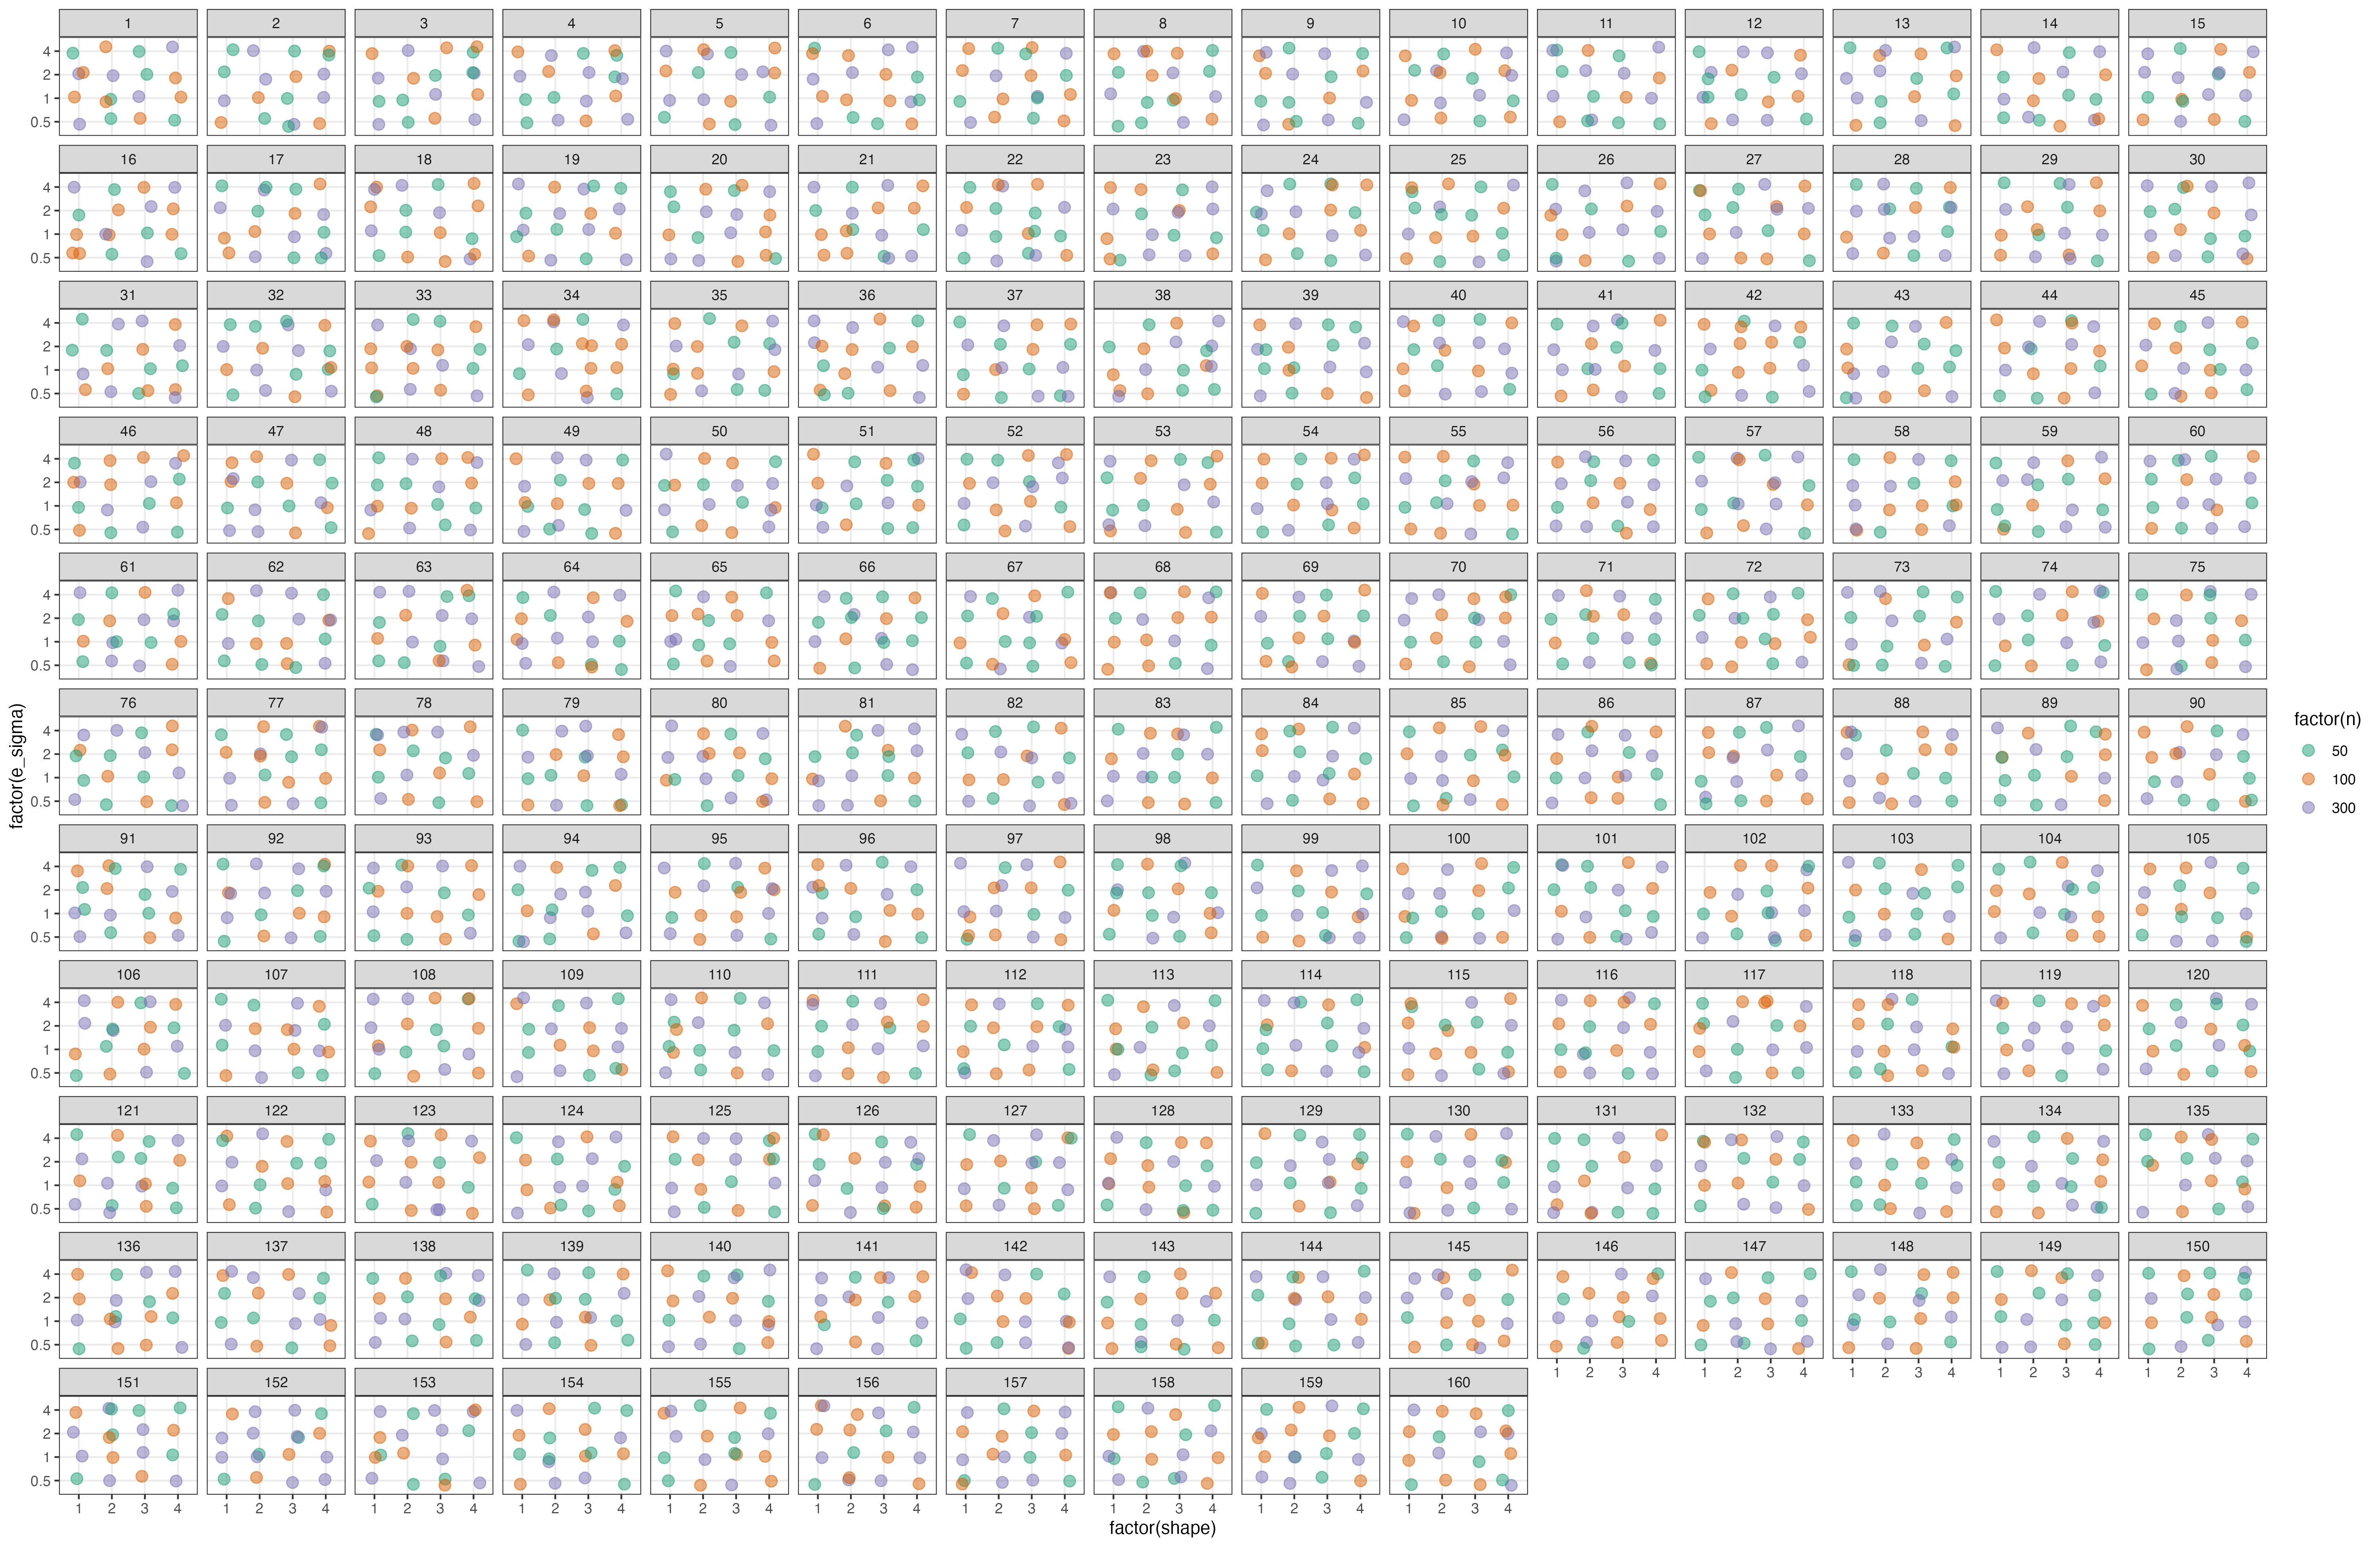
\includegraphics[width=1\linewidth]{figures/check_allocation_for_subject_nonlin} \end{center}

\begin{center}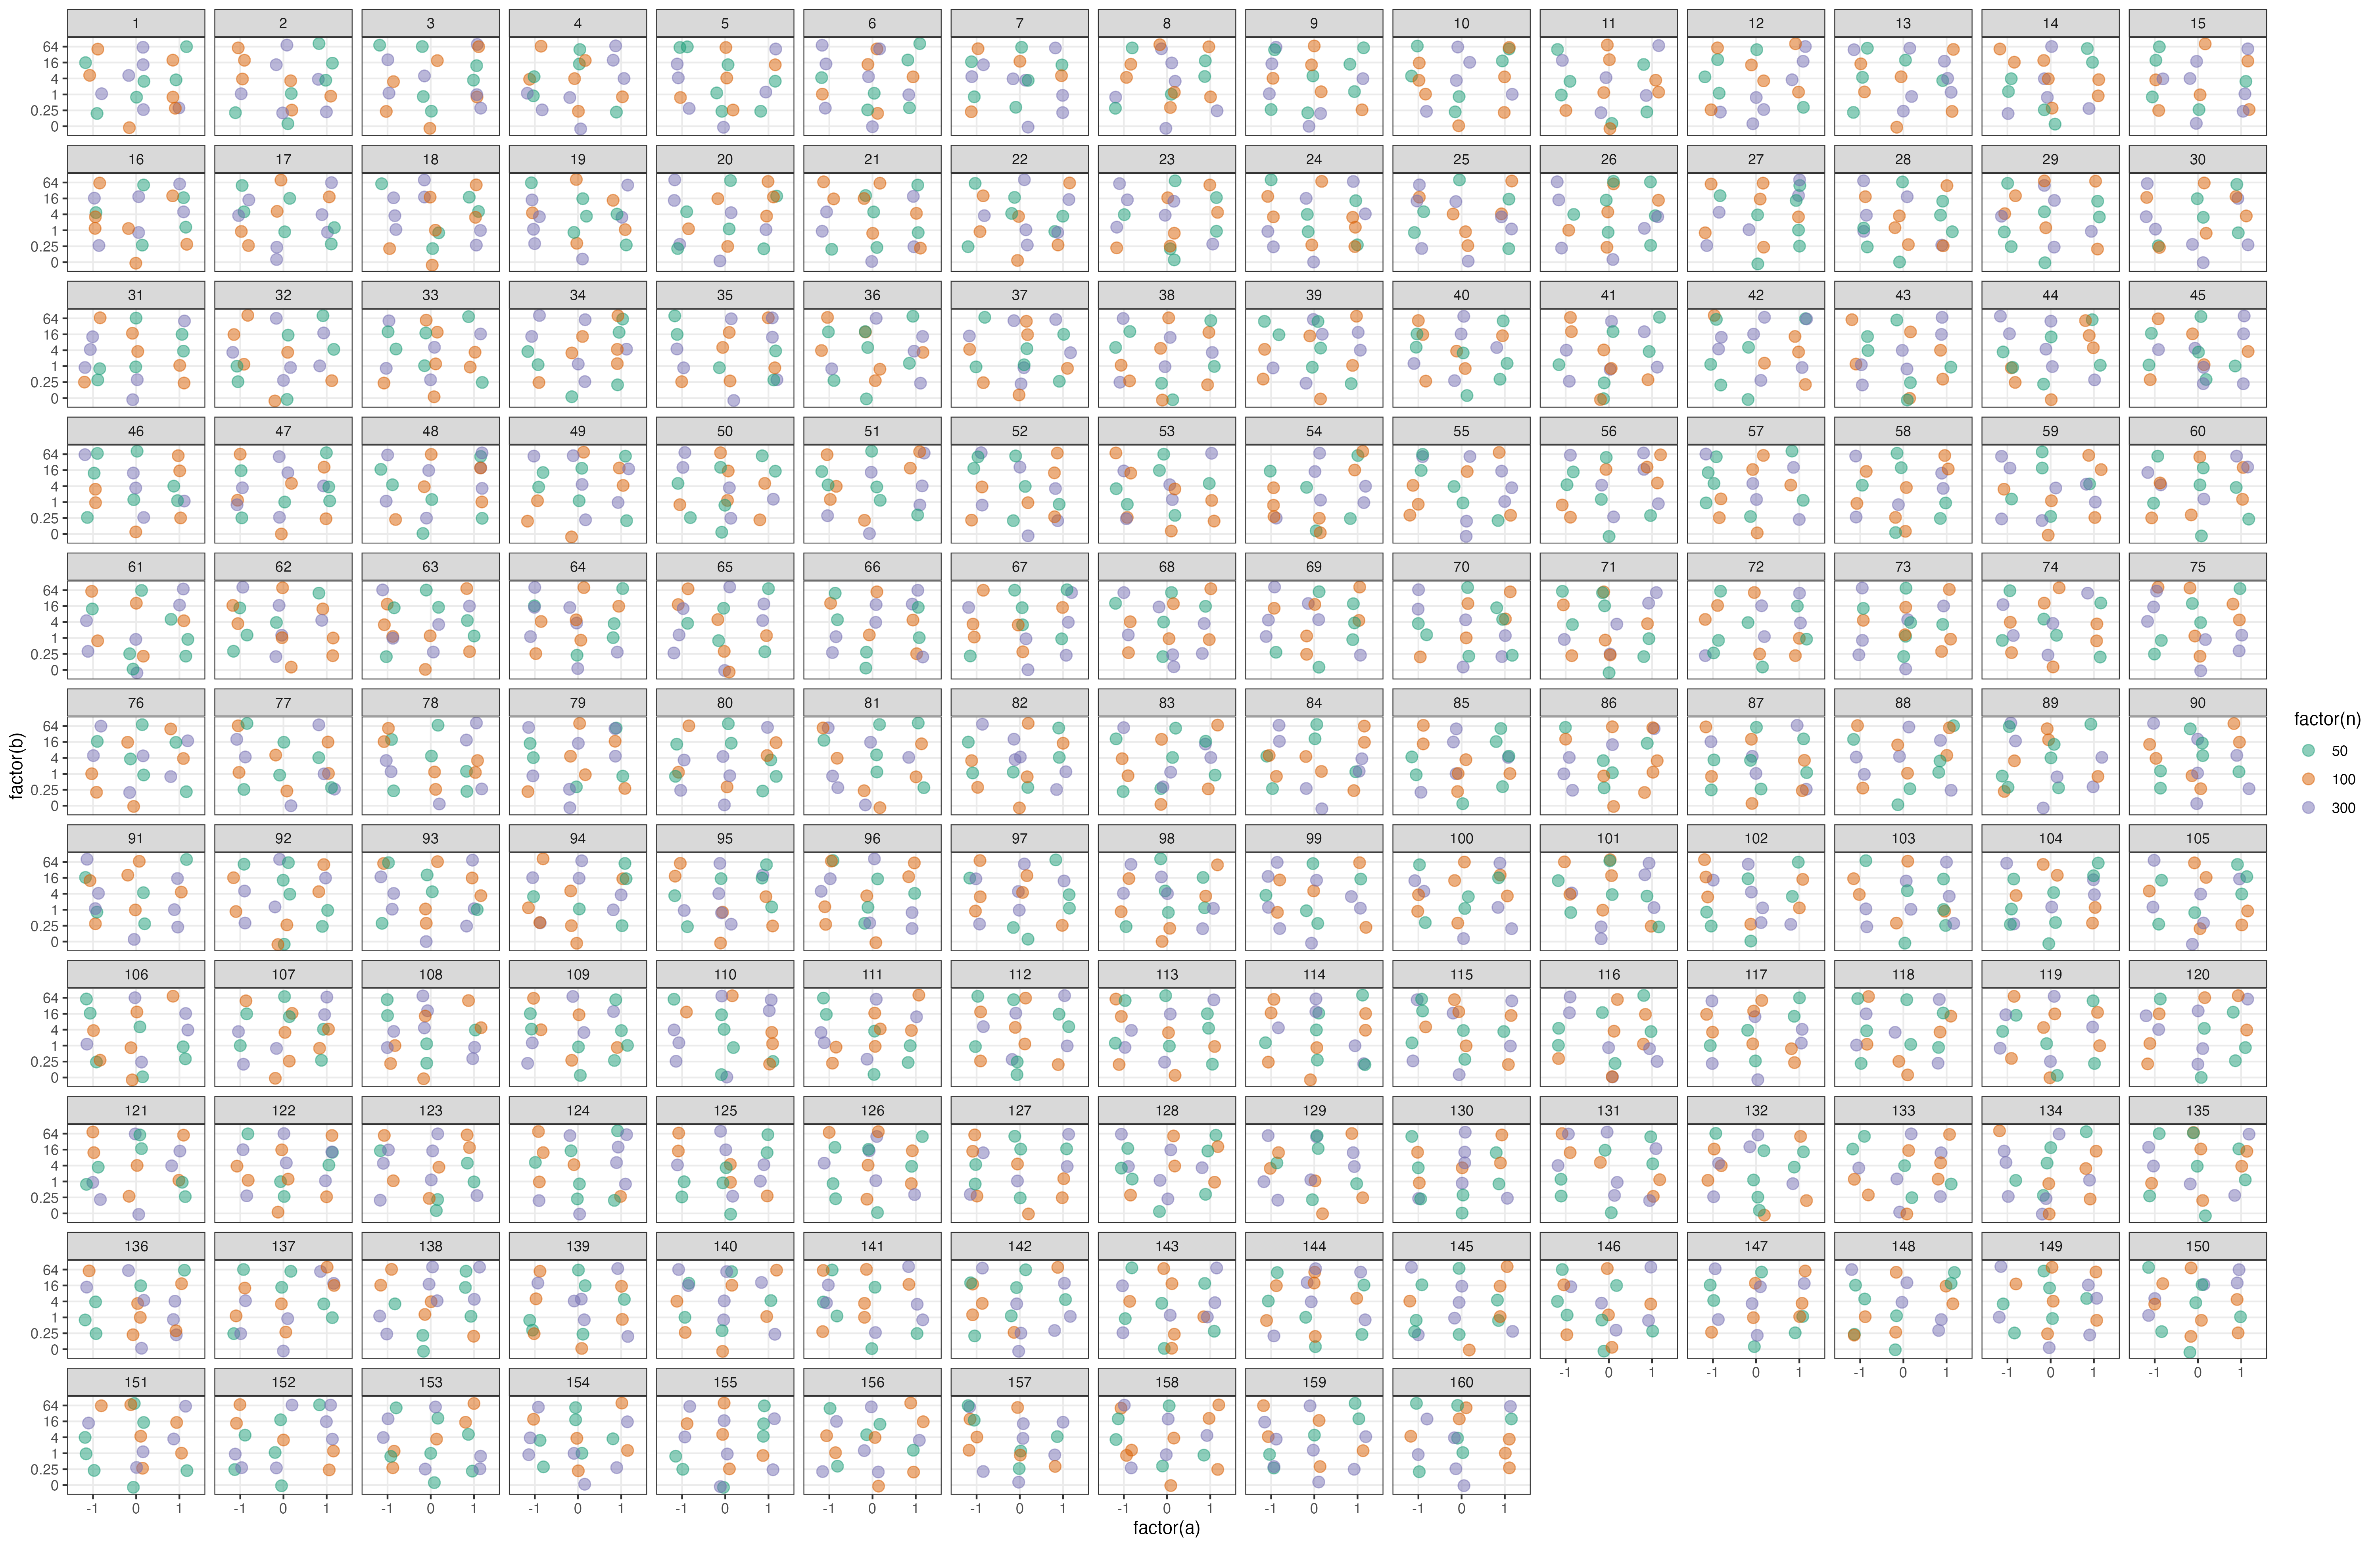
\includegraphics[width=1\linewidth]{figures/check_allocation_for_subject_hetero} \end{center}

\hypertarget{data-collection-process}{%
\subsection{Data collection process}\label{data-collection-process}}

The survey data is collected via a self-hosted website designed by us.
The complete architecture is provided in Figure \ref{fig:tech}. The
website is built with the \texttt{Flask} \citep{flask} web framework and
hosted on \texttt{PythonAnywhere} \citep{pythonanywhere}. It is
configured to handle HTTP requests such that participants can correctly
receive webpages and submit responses. Embedded in the resources sent to
participants, the \texttt{jsPsych} front-end framework \citep{jspsych}
instructs participants' browsers to render an environment for running
behavioral experiments. During the experiment, this framework will
automatically collect common behavioral data such as response time and
clicks on buttons. participants' responses are first validated by a
scheduled \texttt{Python} script run on the server, then push to a
Github repository. Lineup images shown to users are saved in multiple
Github repositories and hosted in corresponding Github pages. The URLs
to these images are resolved by \texttt{Flask} and bundled in HTML
files.

Once the participant is recruited from Prolific
\citep{palan2018prolific}, it will be redirected to the entry page of
our study website. An image of the entry page is provided in Figure
\ref{fig:entry-page}. Then, the participant needs to submit the online
consent form and fill in the demographic information as shown in
\ref{fig:consent-form} and \ref{fig:metadata} respectively. Before
evaluating lineups, participant also need to read the training page as
provide in Figure \ref{fig:training-page} to understand the process. An
example of the lineup page is given in Figure \ref{fig:lineup-page}. A
half of the page is taken by the lineup image to attract participant's
attention. The button to skip the selections for the current lineup is
intentionally put in the corner of the bounding box with smaller font
size, such that participants will not misuse this functionality.

\begin{figure}

{\centering 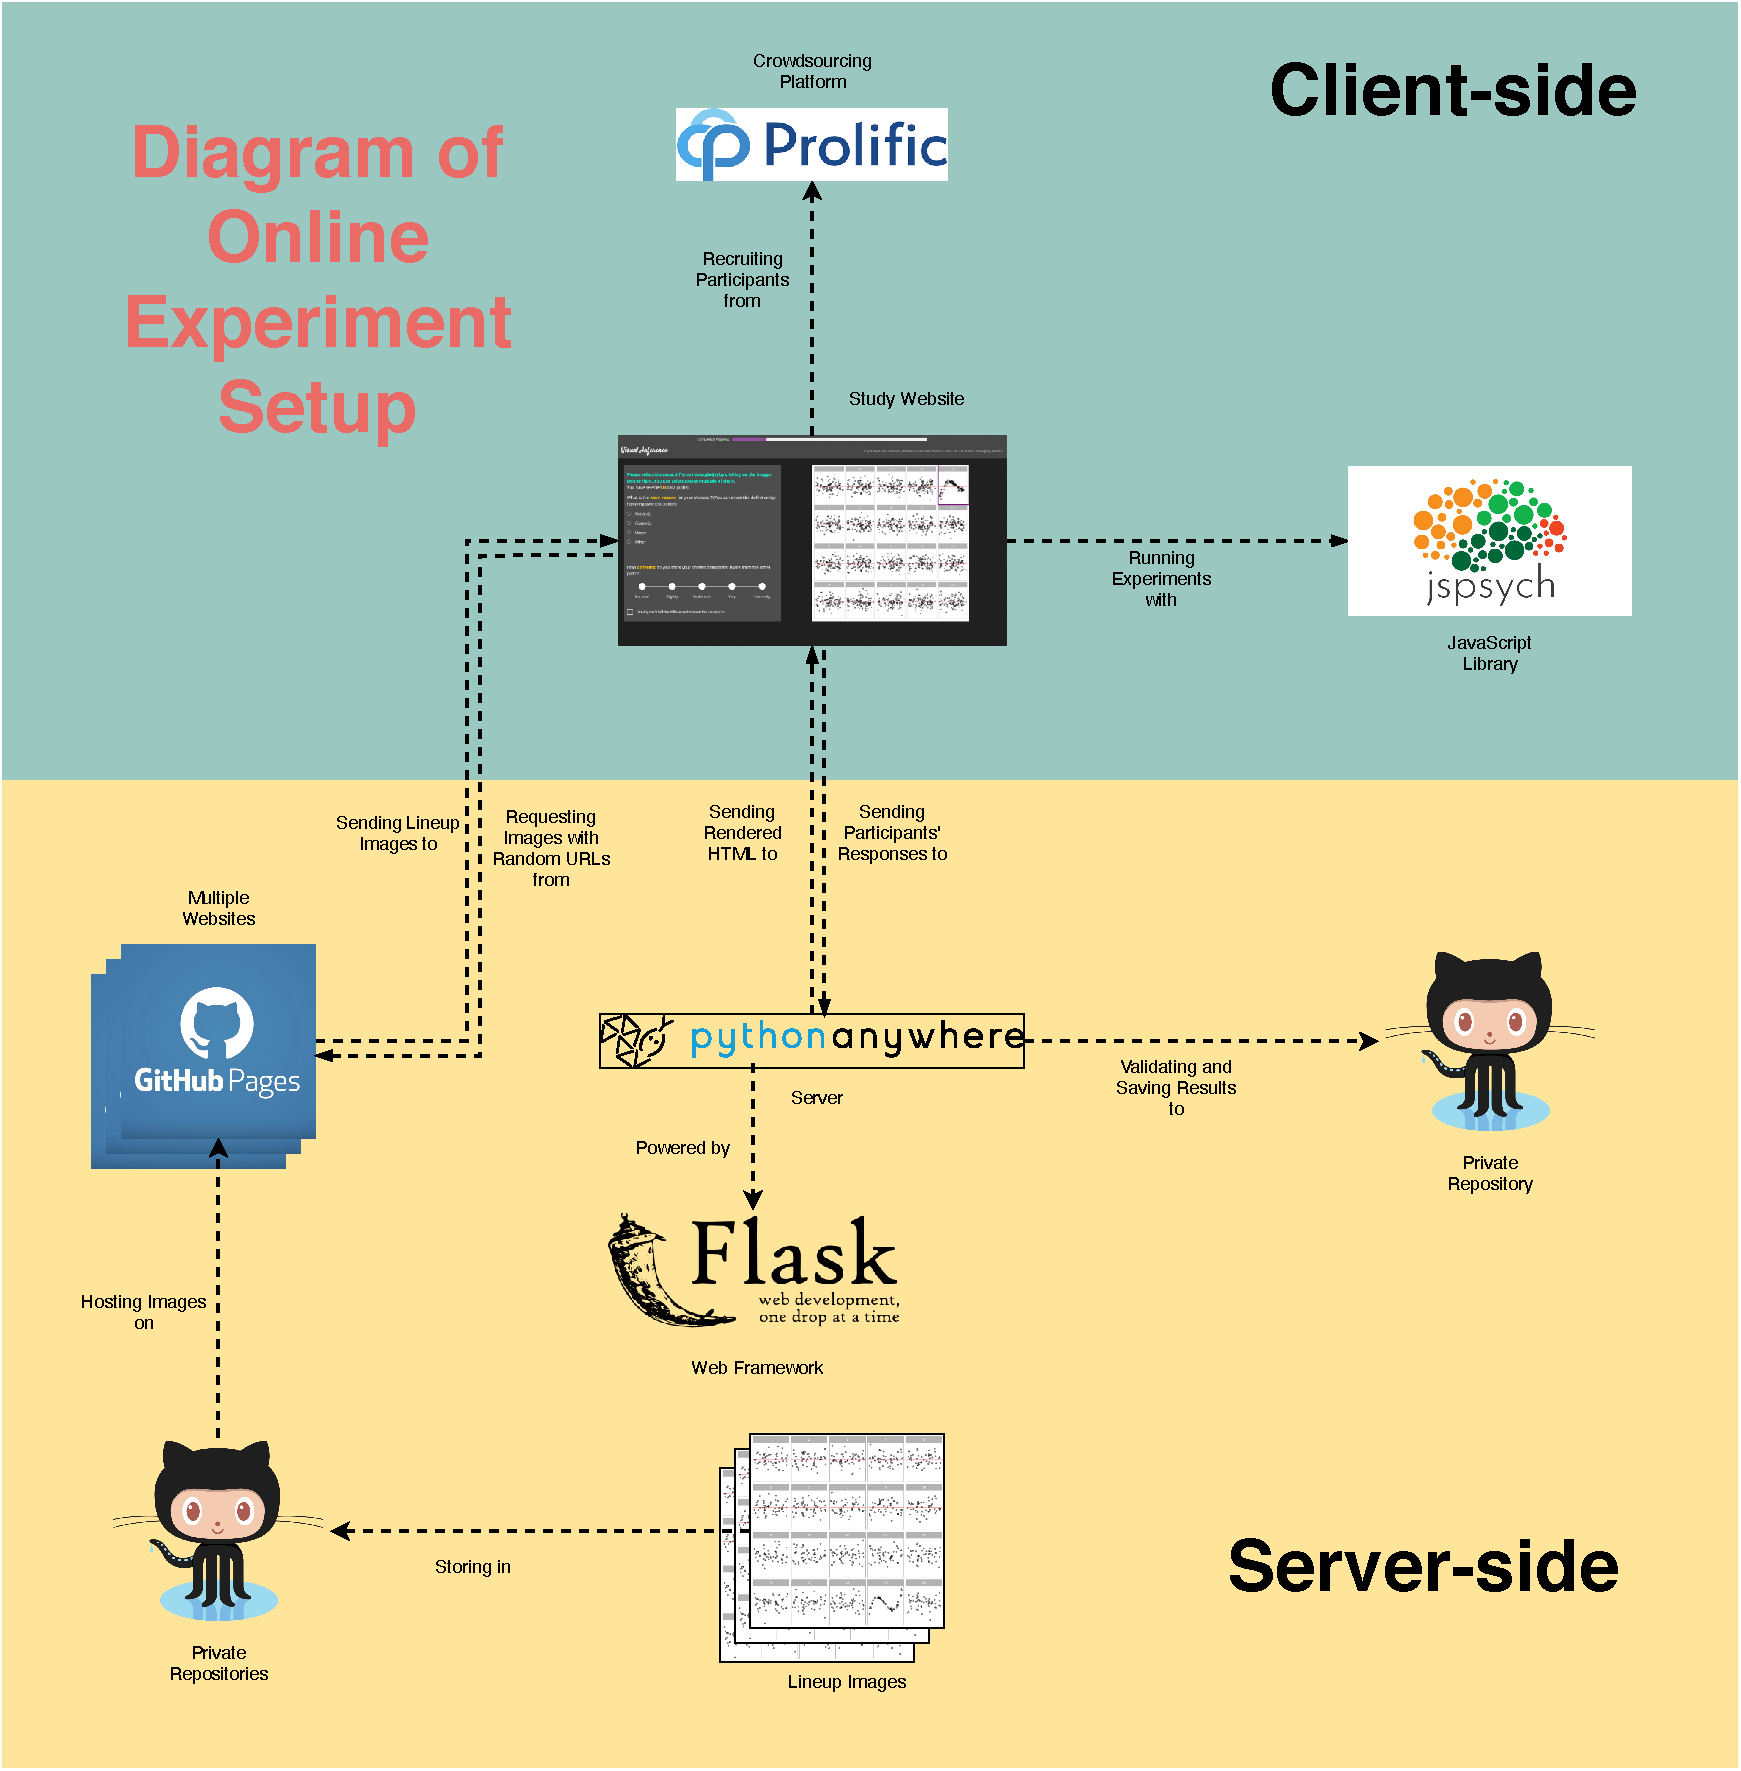
\includegraphics[width=1\linewidth]{figures/experiment_tech} 

}

\caption{Diagram of online experiment setup. The server-side of the study website uses Flask as backend hosted on PythonAnywhere. And the client-side uses jsPsych to run experiment.}\label{fig:tech}
\end{figure}

\begin{figure}

{\centering 
\includegraphics[width=1\linewidth]{figures/message} 

}

\caption{The entry page of the study website.}\label{fig:entry-page}
\end{figure}

\begin{figure}

{\centering 
\includegraphics[width=1\linewidth]{figures/consent_form} 

}

\caption{The consent form provided in the study website.}\label{fig:consent-form}
\end{figure}

\begin{figure}

{\centering 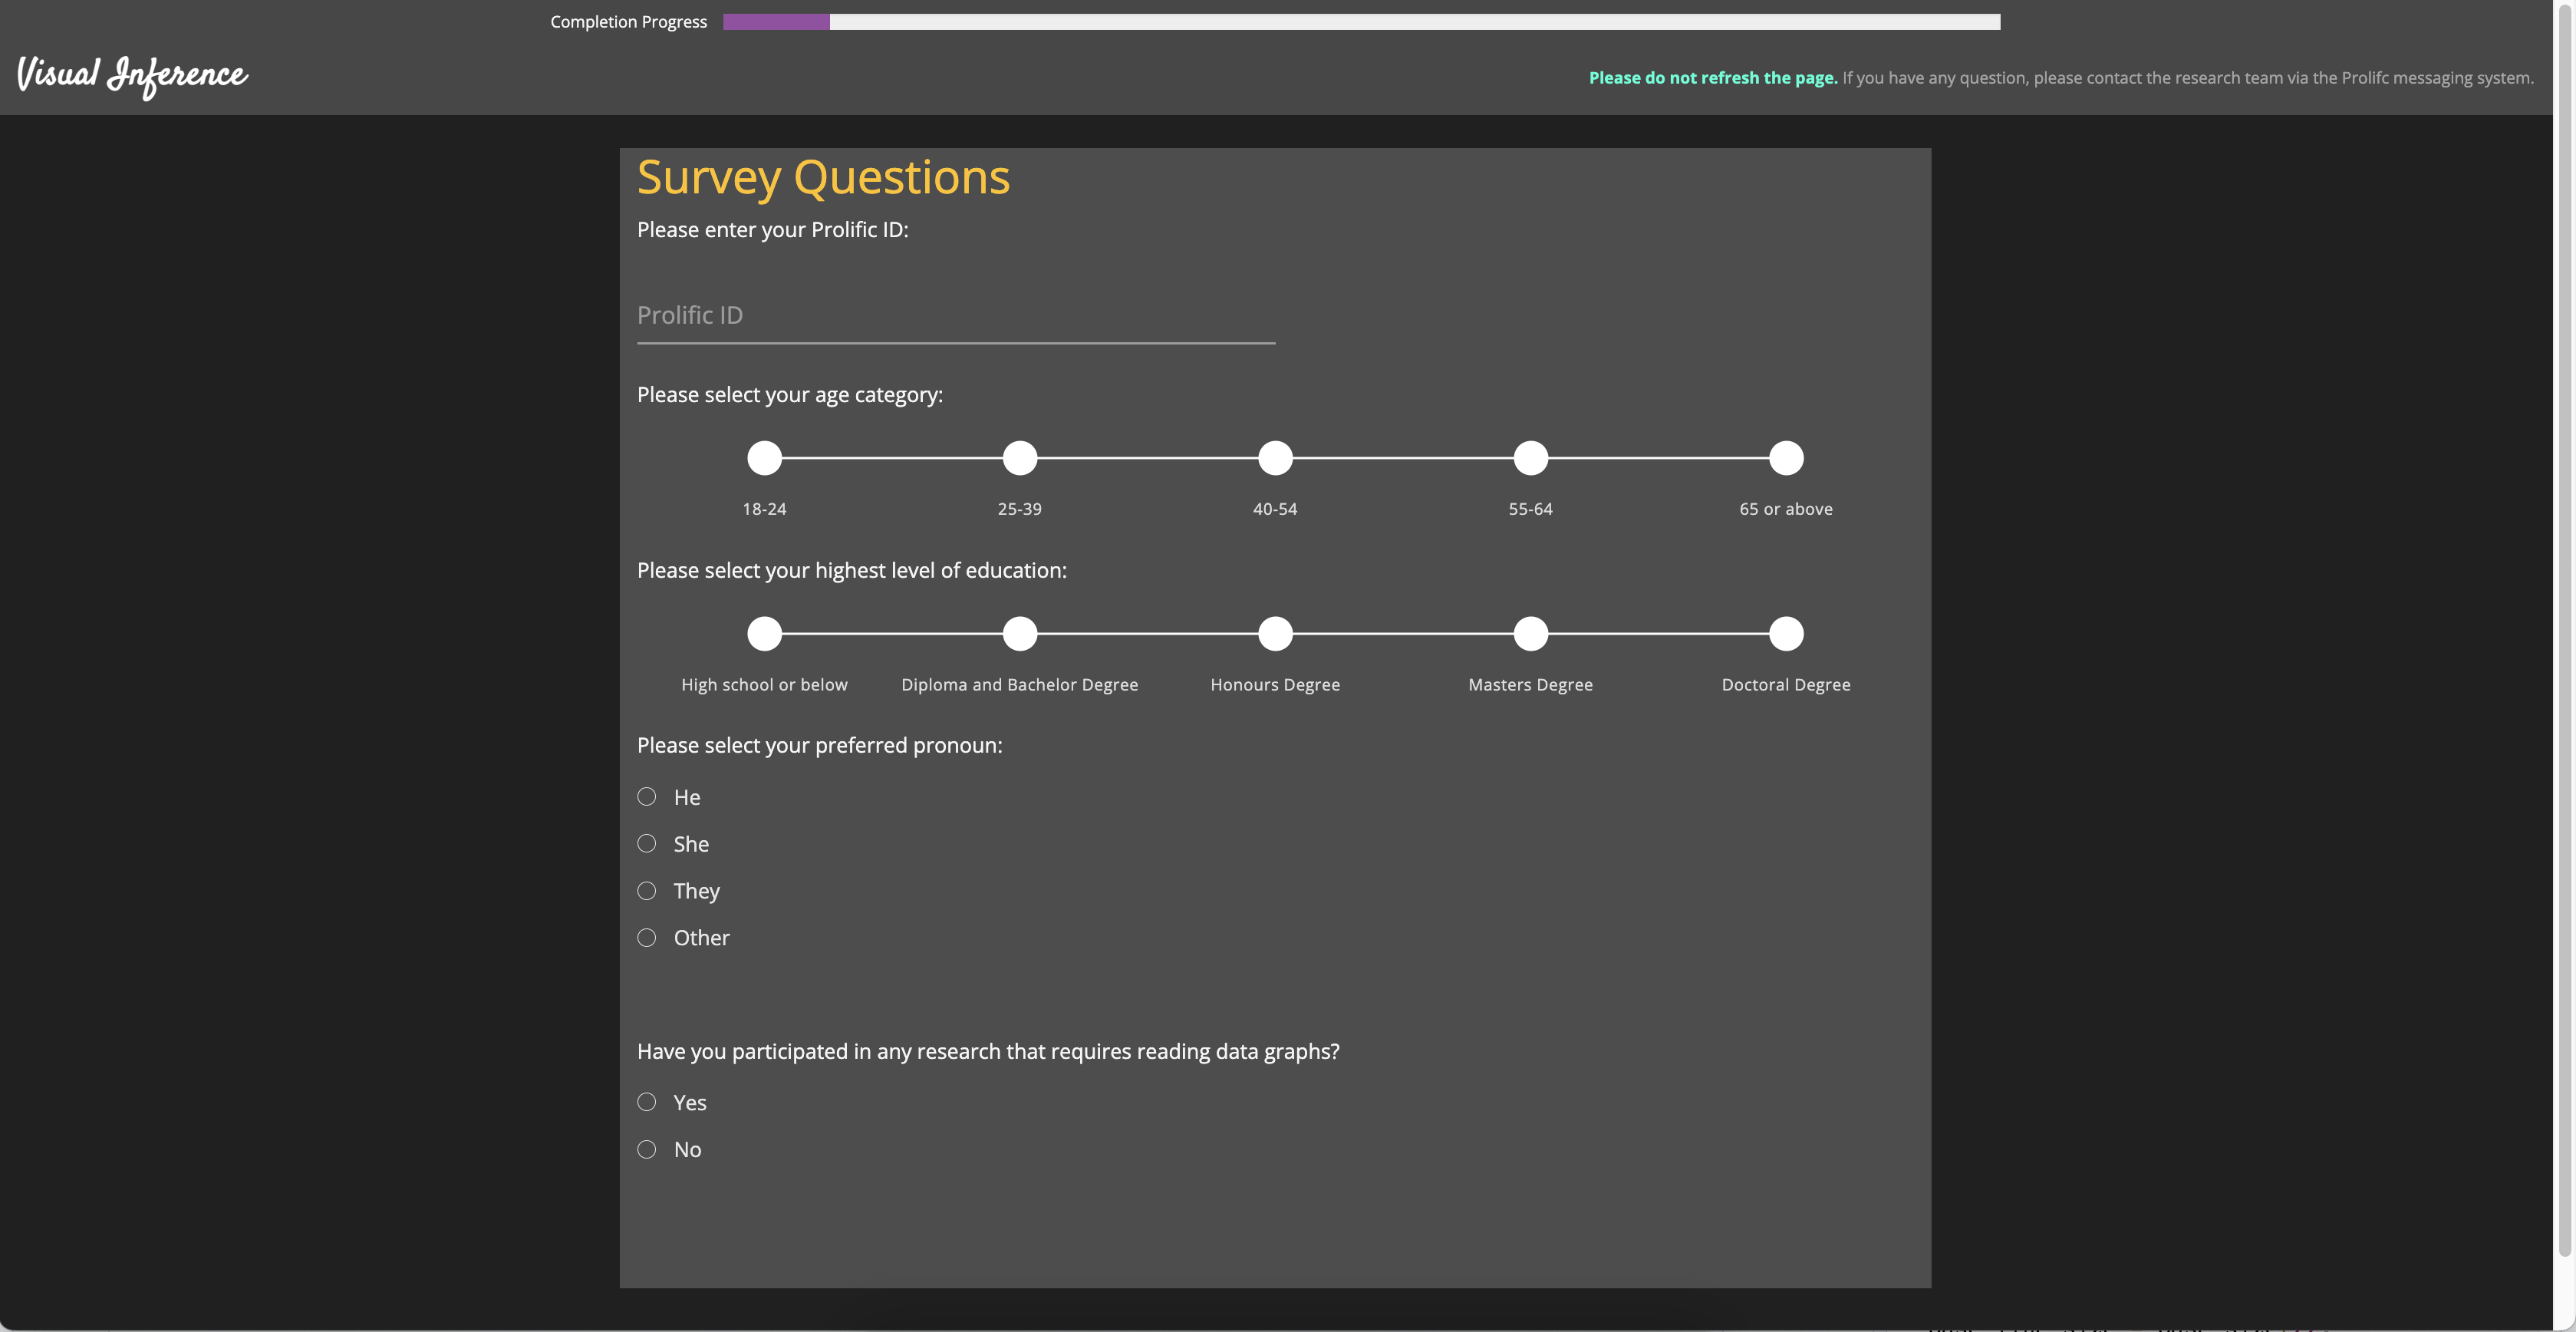
\includegraphics[width=1\linewidth]{figures/metadata} 

}

\caption{The form to provide demographic information.}\label{fig:metadata}
\end{figure}

\begin{figure}

{\centering 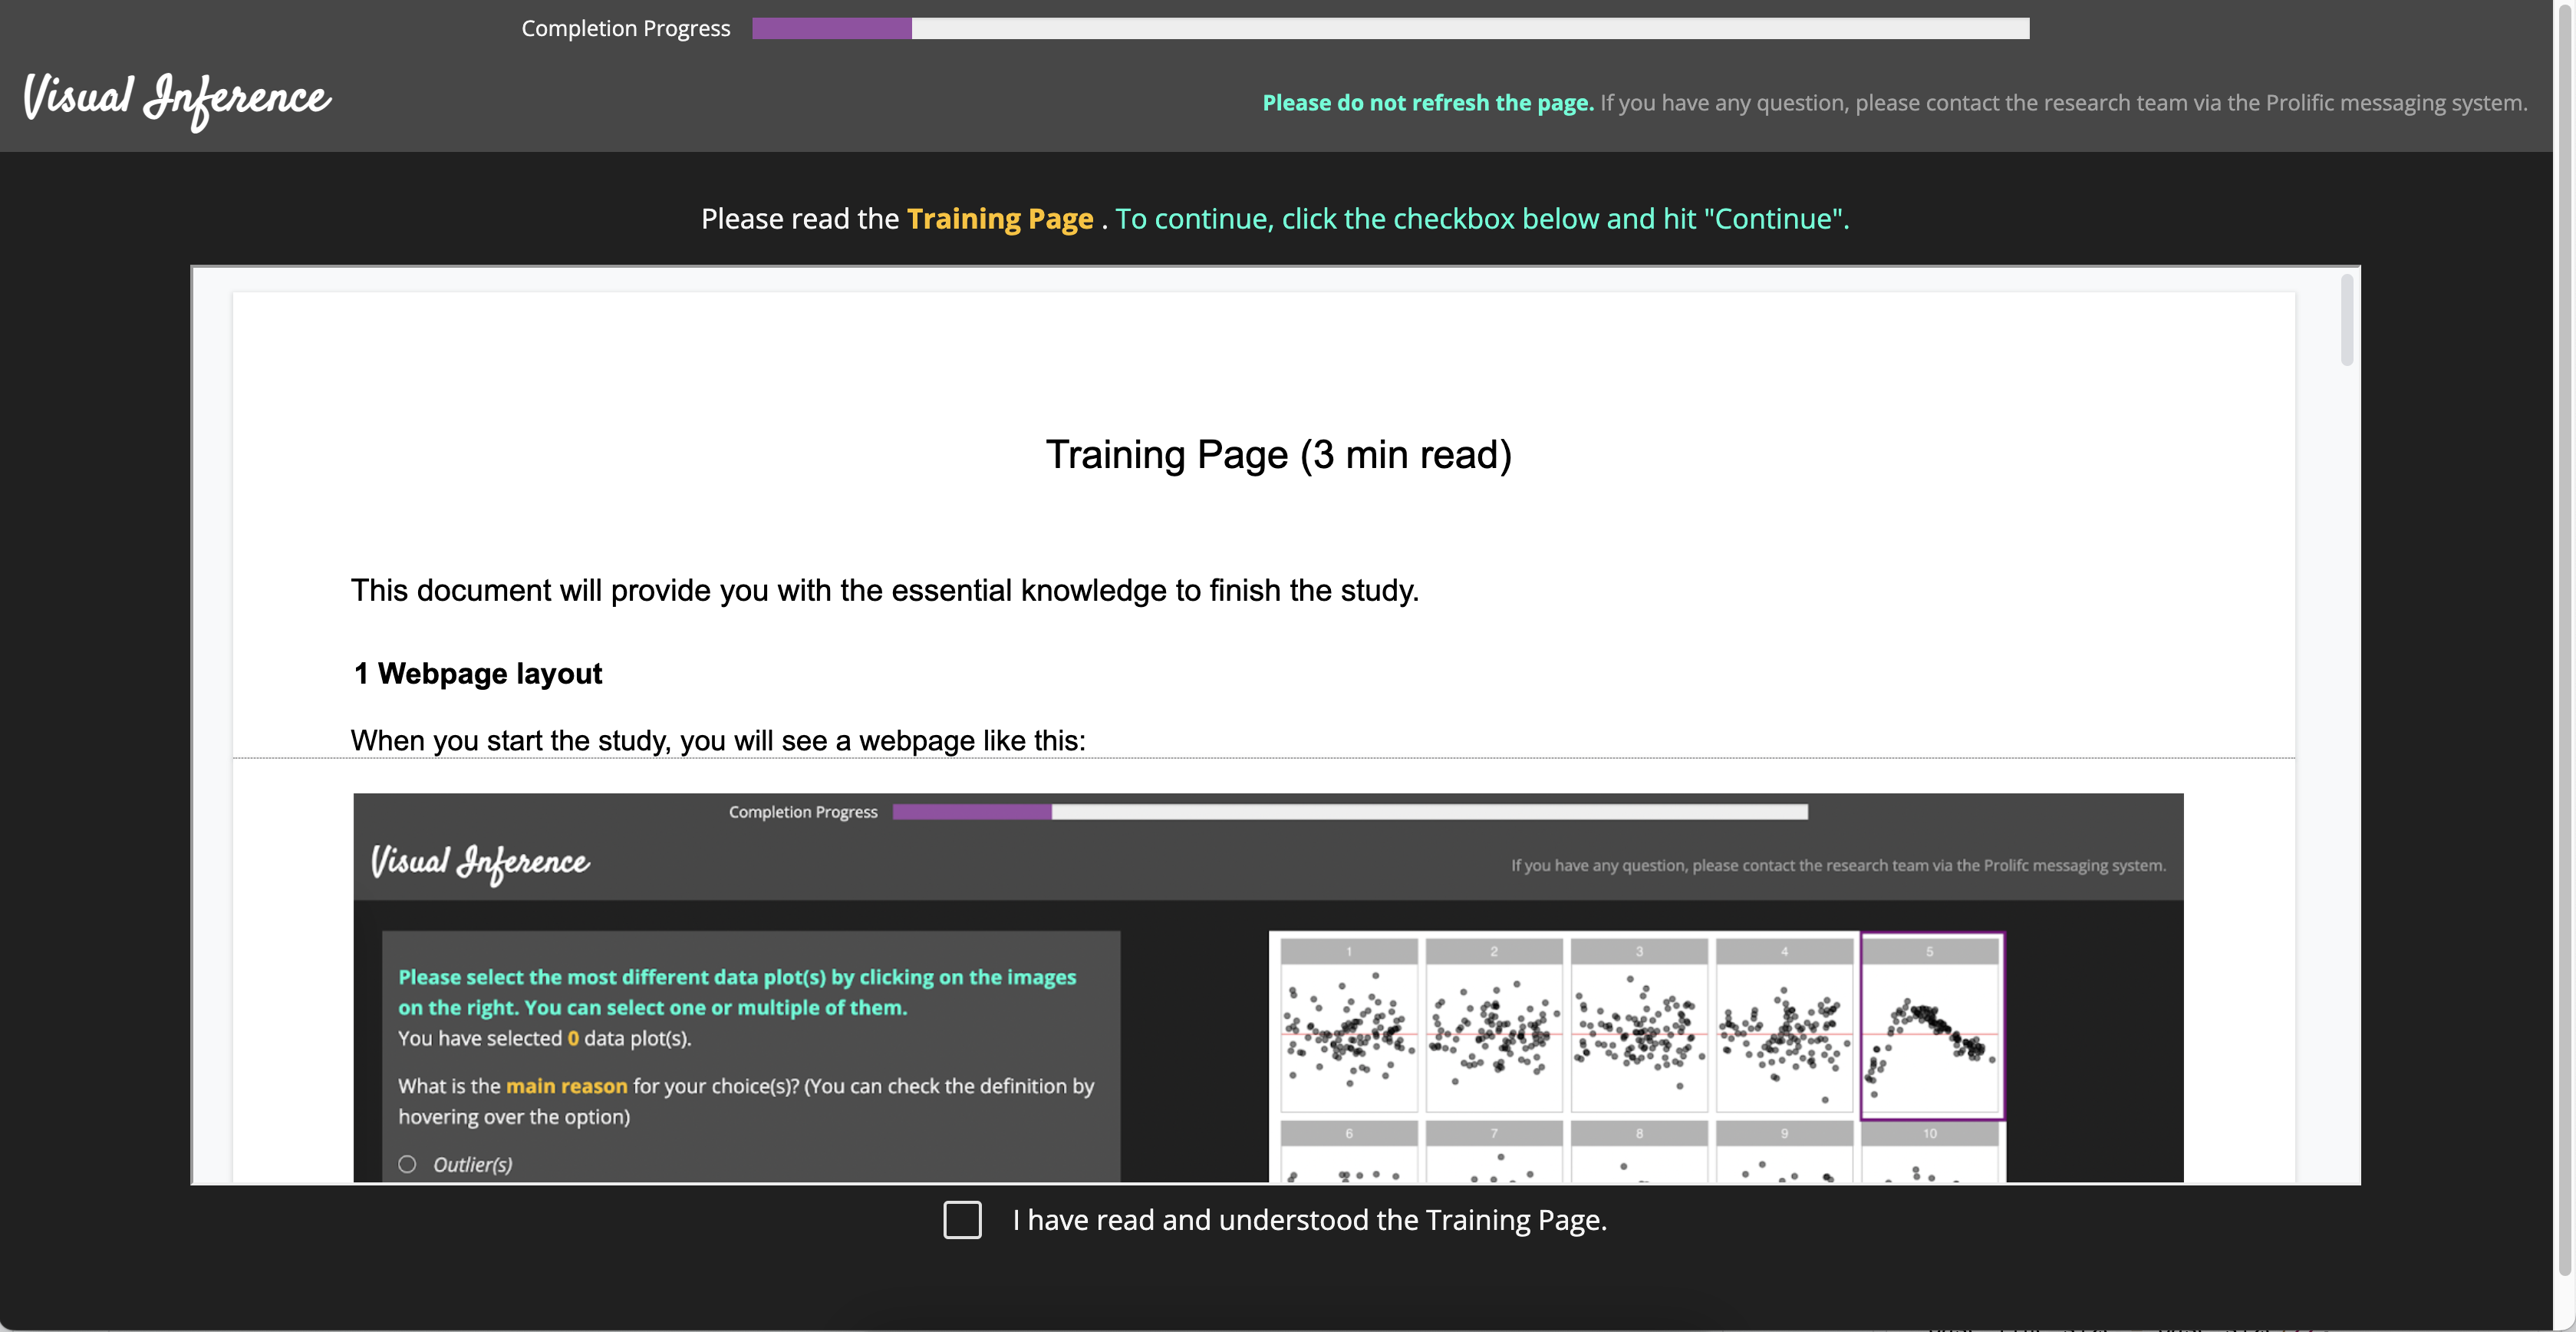
\includegraphics[width=1\linewidth]{figures/training} 

}

\caption{The training page of the study website.}\label{fig:training-page}
\end{figure}

\begin{figure}

{\centering 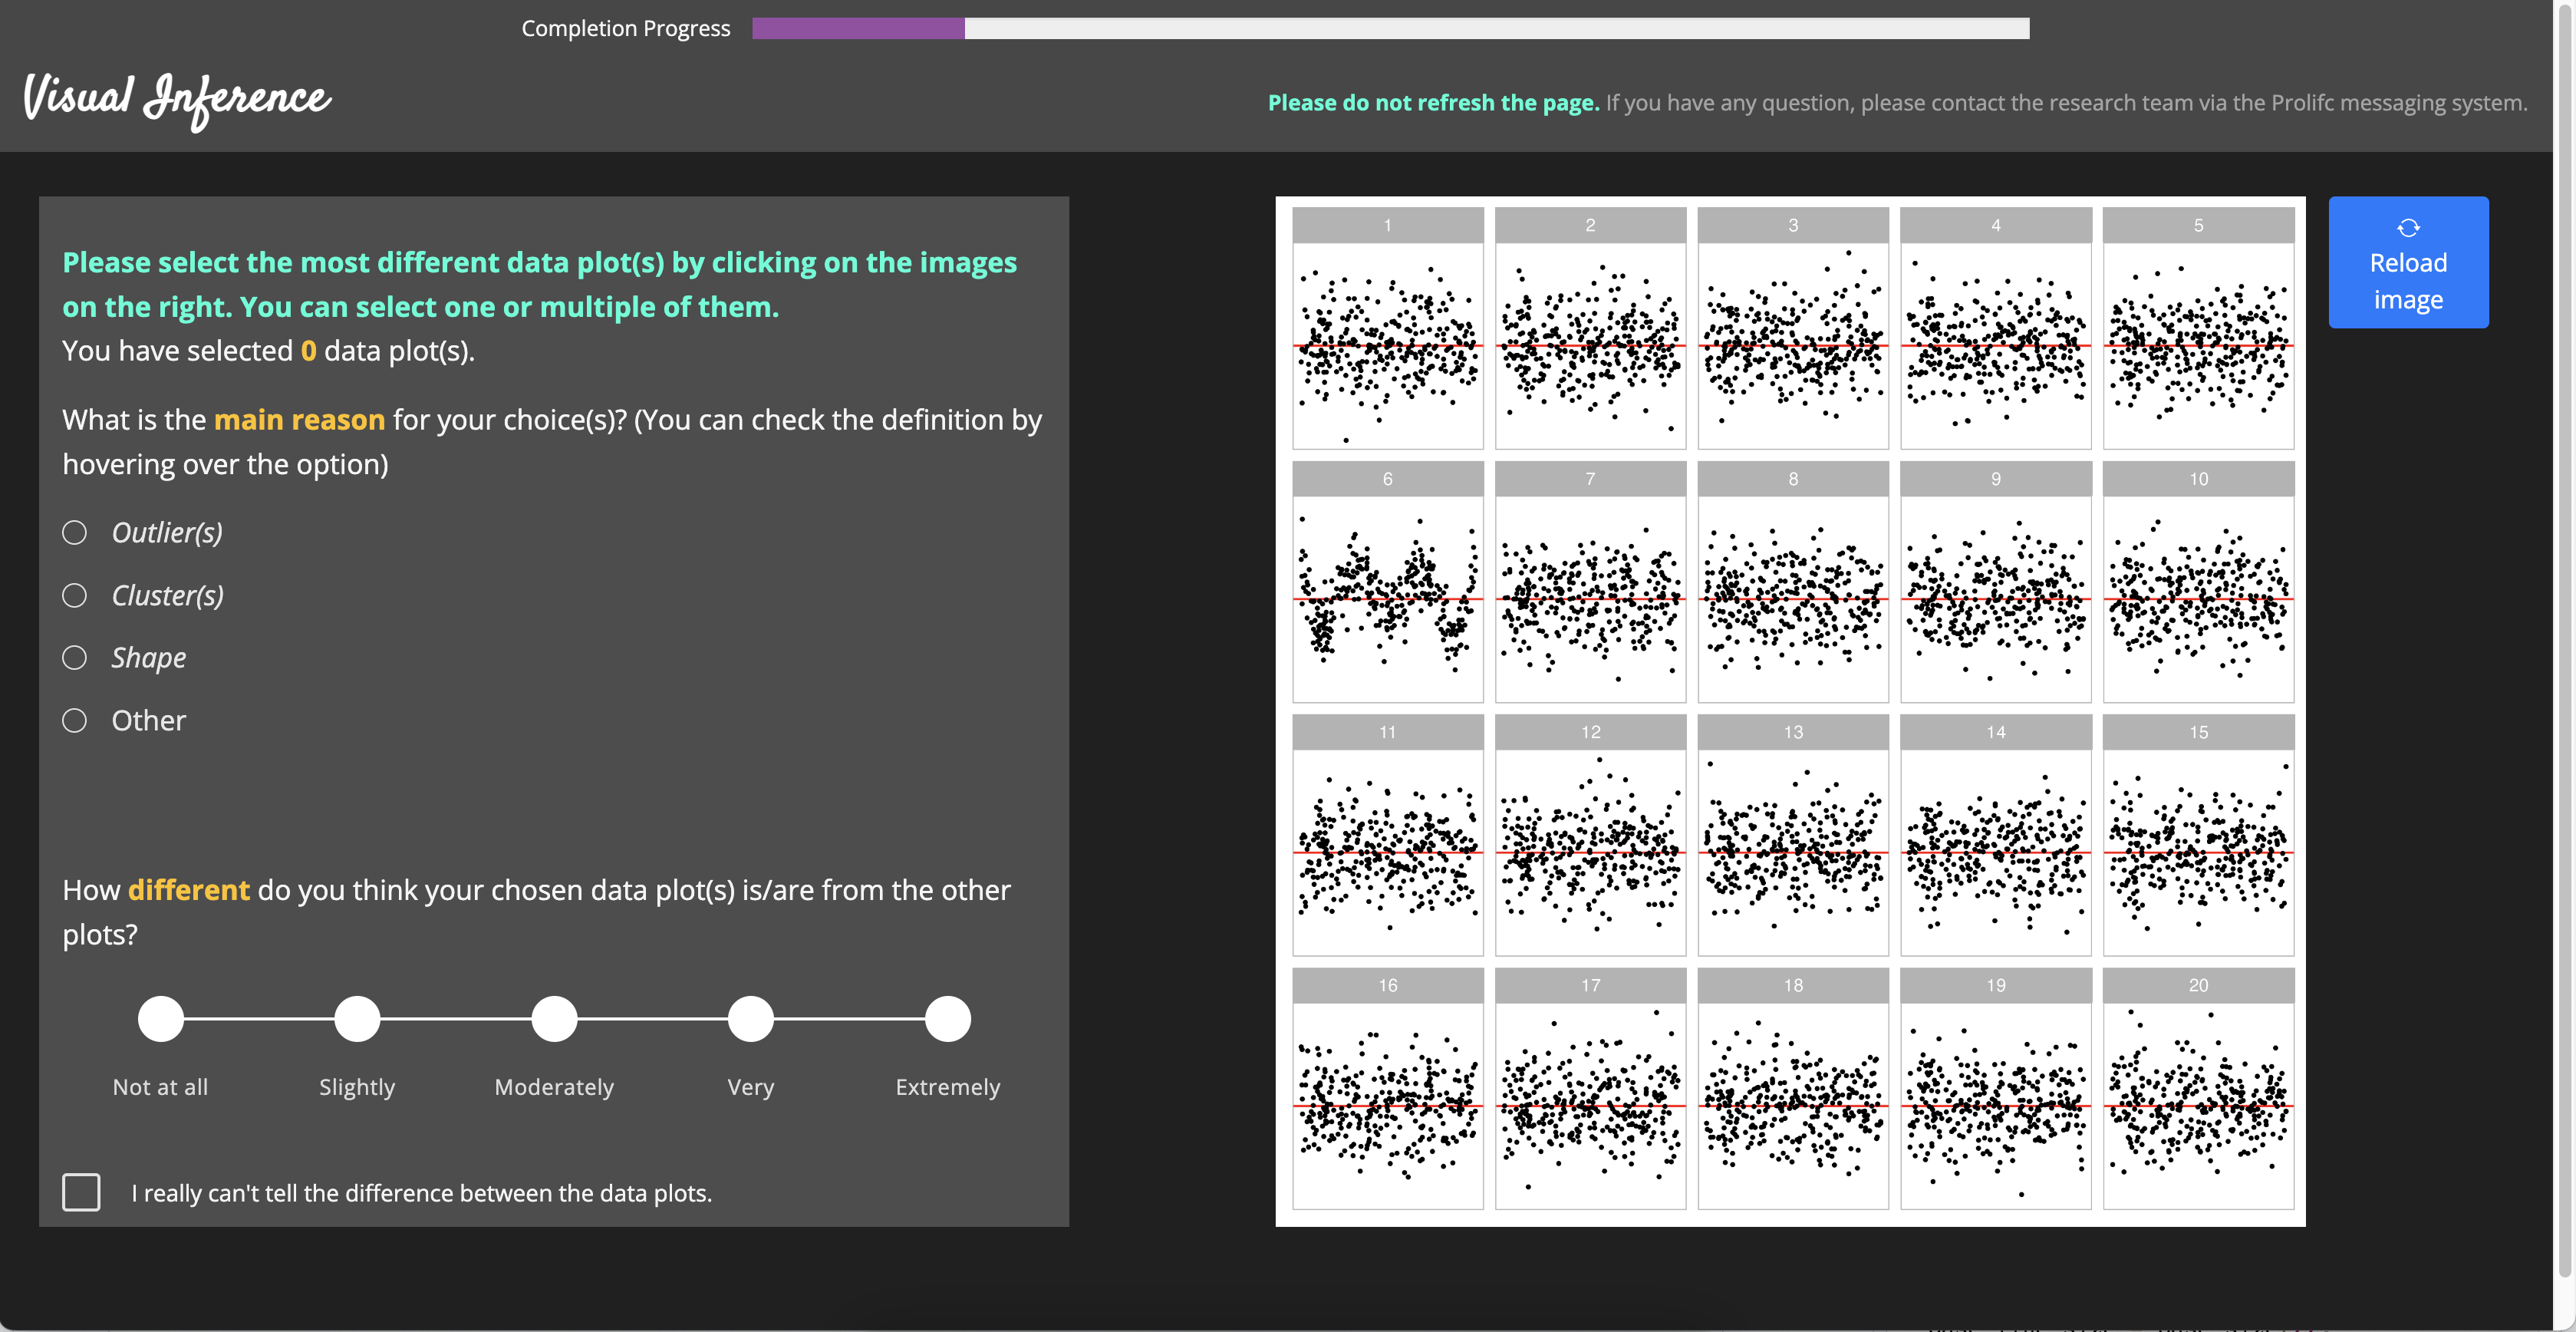
\includegraphics[width=1\linewidth]{figures/lineup1} 

}

\caption{The lineup page of the study website.}\label{fig:lineup-page}
\end{figure}

\newpage

\hypertarget{analysis-of-results-relative-to-data-collection-process}{%
\section{Analysis of results relative to data collection
process}\label{analysis-of-results-relative-to-data-collection-process}}

\hypertarget{demographics}{%
\subsection{Demographics}\label{demographics}}

Throughout the study, we have collected 7254 evaluations on 1116
non-null lineups. Table \ref{tab:count-lineup} gives further details
about the number of evaluations, lineups and participants over pattern
types and data collection periods.

\begin{table}

\caption{\label{tab:count-lineup}Count of lineups, evaluations and participants over departure types and data collection periods.}
\centering
\begin{tabular}[t]{lrrrrrrr}
\toprule
\multicolumn{1}{c}{ } & \multicolumn{3}{c}{Non-linearity} & \multicolumn{3}{c}{Heteroskedasticity} \\
\cmidrule(l{3pt}r{3pt}){2-4} \cmidrule(l{3pt}r{3pt}){5-7}
Number & I & II & III & I & II & II & Total\\
\midrule
Lineups & 576 & 0 & 144 & 0 & 540 & 135 & 1116\\
Evaluations & 2880 & 0 & 864 & 0 & 2700 & 810 & 7254\\
Participants & 160 & 0 & 123 & 0 & 160 & 123 & 443\\
\bottomrule
\end{tabular}
\end{table}

Along with the responses to lineups, we have collected a series of
demographic information including age, pronoun, education background and
previous experience in studies involved data visualization. Table
\ref{tab:pronoun}, \ref{tab:age-group}, \ref{tab:education} and
\ref{tab:experience} provide summary of the demographic data.

It can be observed from the tables that most participants have Diploma
or Bachelor degrees, followed by High school or below and the survey
data is gender balanced. Majority of participants are between 18 to 39
years old and there are slightly more participants who do not have
previous experience than those who have.

\begin{table}

\caption{\label{tab:pronoun}Summary of pronoun distribution of participants recruited in this study.}
\centering
\resizebox{\linewidth}{!}{
\begin{tabular}[t]{lrrrrrrrr}
\toprule
Pronoun & Period I & \% & Period II & \% & Period III & \% & Total & \%\\
\midrule
He & 77 & 17.4 & 79 & 17.8 & 61 & 13.8 & 217 & 49.0\\
She & 78 & 17.6 & 77 & 17.4 & 61 & 13.8 & 216 & 48.8\\
Other & 5 & 1.1 & 4 & 0.9 & 1 & 0.2 & 10 & 2.3\\
 & 160 & 36.1 & 160 & 36.1 & 123 & 27.8 & 443 & 100.0\\
\bottomrule
\end{tabular}}
\end{table}

\begin{table}

\caption{\label{tab:age-group}Summary of age distribution of participants recruited in this study.}
\centering
\resizebox{\linewidth}{!}{
\begin{tabular}[t]{lrrrrrrrr}
\toprule
Age group & Period I & \% & Period II & \% & Period III & \% & Total & \%\\
\midrule
18-24 & 83 & 18.7 & 86 & 19.4 & 51 & 11.5 & 220 & 49.7\\
25-39 & 69 & 15.6 & 63 & 14.2 & 63 & 14.2 & 195 & 44.0\\
40-54 & 6 & 1.4 & 8 & 1.8 & 6 & 1.4 & 20 & 4.5\\
55-64 & 2 & 0.5 & 3 & 0.7 & 3 & 0.7 & 8 & 1.8\\
 & 160 & 36.1 & 160 & 36.1 & 123 & 27.8 & 443 & 100.0\\
\bottomrule
\end{tabular}}
\end{table}

\begin{table}

\caption{\label{tab:education}Summary of education distribution of participants recruited in this study.}
\centering
\resizebox{\linewidth}{!}{
\begin{tabular}[t]{lrrrrrrrr}
\toprule
Education & Period I & \% & Period II & \% & Period III & \% & Total & \%\\
\midrule
High School or below & 41 & 9.3 & 53 & 12.0 & 33 & 7.4 & 127 & 28.7\\
Diploma and Bachelor Degree & 92 & 20.8 & 79 & 17.8 & 66 & 14.9 & 237 & 53.5\\
Honours Degree & 6 & 1.4 & 15 & 3.4 & 6 & 1.4 & 27 & 6.1\\
Masters Degree & 21 & 4.7 & 13 & 2.9 & 16 & 3.6 & 50 & 11.3\\
Doctoral Degree & 0 & 0.0 & 0 & 0.0 & 2 & 0.5 & 2 & 0.5\\
\addlinespace
 & 160 & 36.1 & 160 & 36.1 & 123 & 27.8 & 443 & 100.0\\
\bottomrule
\end{tabular}}
\end{table}

\begin{table}

\caption{\label{tab:experience}Summary of previous experience distribution of participants recruited in this study.}
\centering
\resizebox{\linewidth}{!}{
\begin{tabular}[t]{lrrrrrrrr}
\toprule
Previous experience & Period I & \% & Period II & \% & Period III & \% & Total & \%\\
\midrule
No & 96 & 21.7 & 88 & 19.9 & 67 & 15.1 & 251 & 56.7\\
Yes & 64 & 14.4 & 72 & 16.3 & 56 & 12.6 & 192 & 43.3\\
 & 160 & 36.1 & 160 & 36.1 & 123 & 27.8 & 443 & 100.0\\
\bottomrule
\end{tabular}}
\end{table}

\hypertarget{data-collection-periods}{%
\subsection{Data collection periods}\label{data-collection-periods}}

\begin{figure}

{\centering \includegraphics[width=1\linewidth]{appendix_files/figure-latex/poly-boxplot-lineup-1} 

}

\caption{A lineup of "letter-value" boxplots of weighted propotion of detect for lineups over different data collection periods for non-linearity model. Can you find the most different boxplot? The data plot is positioned in panel $2^3 - 1$.}\label{fig:poly-boxplot-lineup}
\end{figure}

\begin{figure}

{\centering \includegraphics[width=1\linewidth]{appendix_files/figure-latex/heter-boxplot-lineup-1} 

}

\caption{A lineup of "letter-value" boxplots of weighted propotion of detect for lineups over different data collection periods for heteroskedasticity model. Can you find the most different boxplot? The data plot is positioned in panel $2^4 - 2$.}\label{fig:heter-boxplot-lineup}
\end{figure}

We have the same type of model collected over different data collection
periods, that may lead to unexpected batch effect. Figure
\ref{fig:poly-boxplot-lineup} and \ref{fig:heter-boxplot-lineup} provide
two lineups to examine whether there is an actual difference across data
collection periods for non-linearity model and heteroskedasticity model
respectively. To emphasize the tail behaviour and display fewer
outliers, we use the ``letter-value'' boxplot \citep{hofmann2017value}
which is an extension of the number of ``letter value'' statistics to
check the weighed proportion of detect over different data collection
period. The weighted proportion of detect is calculated by taking the
average of \(c_i\) of a lineup over a data collection period. Within our
research team, we can not identify the data plot from the null plots for
these two lineups, result in \(p\)-values much greater than \(5\)\%.
Thus, there is no clear evidence of batch effect.

\bibliographystyle{tfcad}
\bibliography{paper.bib}





\end{document}
